\documentclass[10pt,        % Don't change the font size!
               a4paper,     % Don't change the paper size!
               journal,     % Journal paper format
%               draft       % Enable this parameter to get a draft version.
               ]{IEEEtran}
\makeatletter

\def\markboth#1#2{\def\leftmark{\@IEEEcompsoconly{\sffamily}\MakeUppercase{\protect#1}}%
\def\rightmark{\@IEEEcompsoconly{\sffamily}\MakeUppercase{\protect#2}}}
\makeatother

% Packages
%\usepackage[latin1]{inputenc}
\usepackage[utf8]{inputenc}
\usepackage[T1]{fontenc}
\usepackage{xcolor}
\usepackage{graphicx}
\usepackage{subcaption}

% \graphicspath{{../pdf/}{../jpeg/}}
% \DeclareGraphicsExtensions{.pdf,.jpeg,.png}

\begin{document}

% paper title
\title{Neural Architecture Search and tinyML: A Survey}
\author{Daniel~Duclos-Cavalcanti}

% The paper headers
\markboth{Seminar for VLSI Entwurfsverfahren, Summer Term 2022}%
{Daniel Duclos-Cavalcanti: Network Architecture Search (NAS)}

% make the title area
\maketitle

%\thanks{Daniel D-C. is with the Department
%of Electrical and Computer Engineering, Technical University of Munich, Bavaria, DE.}% <-this % stops a space

\begin{abstract}
There is no denying the increasing success that Deep Neural Networks (DNNs)
have displayed across various tasks such as speech recognition, image classification
and many others. This progress can be attributed largely due to \textit{architecture engineering},
which is a process that requires immense domain expertise, intuition and some amount of trial
and error. This is not ideal as it is both time consuming and error-prone. Neural Architecture Search (NAS)
rises as the next logical step aiming to automate architecture discovery.
This field has grown remarkably within the last 5 years and was able to, through
many optimizations, obtain competetive architectures with accuracies that rival state of the art models.
This however changes within the context of \textit{tinyML}, which is an expanding field at the intersection of
machine learning and embedded systems.
Due to the resource-constrained conditions involved in most embedded devices, there are other goals other than inference
accuracy such as latency, energy consumption, memory consumption, and many others to consider. Generally, the manual
process to port AI algorithms on said devices include not only training a given NN, but also pruning, quantizing and
in some cases designing custom hardware to implement said model. This approach typically includes not optimal
solutions due to the mutual influence of the hardware and algorithm.
Given the extensive work done on NAS in the last years, there has been interesting efforts that
utilized existing NAS algorithms to optimize a model's search considering these many other dimensions to best fit a
given hardware platform or device in an automated fashion.
Throughout this work, an overview of existing research in NAS, specifically concerned
with the use of evolutionary algorithms methods will be presented, as well as briefly highlighting
relevant applications within tinyML.

\end{abstract}

\begin{IEEEkeywords}
Neural Architecture Search (NAS), evolutionary computation (EC), Deep Learning, tinyML.
\end{IEEEkeywords}

\section{Introduction}
The advancement of deep learning, although extremely beneficial, has also caused a continuous demand for
architecture design. This coupled with a growing model complexity, demands ample time and expert knowledge to
either improve existing architectures or create new ones for novel applications or problems.


After the work in \cite{zoph2016neural} proposed by Google, it was shown for the first time that NAS algorithms
have the potential to find models that rival the current state of the art. However, done so in an automated fashion and minimizing
human participation. Since then, many different methods have appeared.

To better understand NAS, one can categorize it using the following characteristics \cite{elsken2019neural}:
\begin{itemize}
    \item \textbf{Search Space}: What is the set of all possible architectures that can in principle be considered
    by the algorithm.

    \item \textbf{Search Strategy}: How the \textit{search space} is explored by the algorithm.

    \item \textbf{Performance Estimation Strategy}: How performance is evaluated at every architecture iteration.
\end{itemize}

\subsection{Search Space}
\label{search}
NAS is an optimization problem, whose search space is the defining factor to its complexity.
The smaller the search space is, the faster the search may converge,
as well as requiring less computational resources. However, this limits the freedom to
explore architectures that have not been conceived before, and also possibly restricts the complexity of the design.

How an architecture is constructed or described is a core concept to how the search space of an NAS algorithm is defined.
Defining an architecture as a \textit{chain-structured neural network}, which essentially consists of a
sequence of layers whose inputs are the output of their preceding layer is over-simplified and a non-realistic approach.
Multiple layer connections and other modern design elements such as skip connections are needed to formulate architectures
capable to deal with complex data sets. This has already been seen in the works of \cite{zoph2016neural} and \cite{pmlr-v70-real17a}
for example.
This allows one to build \textit{multi-branch networks}, which are structures where each layer's input is a function of
previous layers outputs, increasing significantly the degrees of freedom of architecture design and the search space's complexity.
The predominant trends are however to search within constructs such as \textit{cells} and \textit{blocks}.

Cells were initially considered by works such as \cite{zhong2018practical} and \cite{zoph2018learning}. What is proposed there,
is to break-off architectures into cells, such that
the search space is then designated within a single cell instead of an entire architecture. This cell is the basic unit of the
resulting architecture, which can be then combined with other identical cells in various fashions to produce a final design.
This strongly reduces the search space, as there are substantially less layers within a single cell in comparison to
an entire architecture. Cells drive the discussion between \textit{micro-architectures} versus \textit{macro-architectures}
\cite{elsken2019neural}. The macro architecture
attempts to determine how cells should be connected and how many are needed to build a model \cite{elsken2019neural}. On the other hand, the micro
architecture aims to find the optimal structure within a cell \cite{elsken2019neural}. Ideally, both should be optimized simultaneously, which of course
leads to a complex search space. There have been efforts to minimize this endeavor by fixing macro-architectures with
known working topographies such as in \cite{pmlr-v80-cai18a} with DenseNet \cite{Huang_2017_CVPR}. This practice, dubbed as
\textit{human knowledge injection} attempts to reduce the search space through applying domain expertise known to obtain good
results.

Search within blocks, similarly to cells, consist of using blocks as basic units of the search space. The difference is that
various layers of different types
are combined to produce basic blocks such as ResBlock, DenseBlock, ConvBlock and so on. These blocks are fixed in their topology
and require less parameters to build an architecture. Therefore, they drastically reduce the search space. Various blocks can be combined
in different manners and quantities to produce competetive architectures. Cells can be considered as a special case of block-based
search, where each block is identical \cite{liu2021survey}.

\subsection{Search Strategy}
As any space search problem, there is a \textit{exploration-exploitation} trade-off to be considered \cite{elsken2019neural}.
Obtaining a high-performing architecture within a feasible amount of time is desired. However, converging too early to a
suboptimal result is also not the goal.

Based on the current state of the art, NAS search algorithms can be classified mainly intro three different
categories \cite{liu2021survey}:

\subsubsection{\textbf{Reinforcement Learning} (RL)-based NAS Algorithms}
Here, one considers the development of a neural architecture as the agent's action, where the action space is the same as
the search space. Therefore, it is then possible to frame NAS as a reinforcement learning problem \cite{elsken2019neural}.
After evaluating the performance of the given trained architecture on fitness data, it is possible to
determine the agent's reward. How this estimation is performed will depend on the given method. Furthermore,
how the agent's policy is represented and it's optimization will also vary.

\subsubsection{\textbf{Evolutionary Computation} (EC)-based NAS Algorithms}
By the application of well established EC methods, which are various techniques based on the evolution of
species within nature, many different efforts were implemented to navigate their respective search space.
More on these different techniques will be seen in section \ref{EV}.

% \textcolor{red}{
% Among others, genetic algorithms (GAs), genetic programming (GP) and particle swarm optimization (PSO)
% techniques have already been successfully applied.
% }

\subsubsection{\textbf{Gradient}-based NAS Algorithms}
EC and Reinforcement learning methods consider an approach, where neural architectures
are spread across a discrete and non-differentiable search space. There are many reasons for this, as networks may differ
through many different manners other than numerical parameters or weights. Gradient-based approaches however
impose restrictions and reformulate the problem to obtain a continuous search space. This allows an algorithm
to use gradient-based methods to pursue an optimal model, which leads many times to competetive and fast techniques.

%% \textcolor{red}{
%% Consists of transforming the search space from discrete to continuous and performing
%% gradient descent with respect to the fitness data set. This transformation requires a set of conditions
%% and has still not been mathematically proven \cite{liu2021survey}.
%% }

\subsection{Performance Estimation Strategy}
\label{PES}
Evaluating the performance of a given architecture is crucial to guide the next steps of the algorithm, regardless of the search
strategy. There are many ways to estimate said performance, whereas the simplest would be complete training and validation.
However, given the complexity and size of the search spaces within most NAS formulations, this
may require GPU days in the order of thousands \cite{elsken2019neural}.
This is why extensive research has been
employed to reduce time on performance estimation, since it is a significant time bottleneck.
Some of these approaches include \cite{elsken2019neural}:
\begin{itemize}
    \item \textbf{Lower Fidelity Techniques}: Shorter training time \cite{zela2018towards}, \cite{zoph2018learning}, training solely on a
        subset of the data \cite{klein2018towards}, training on downscaled data \cite{chrabaszcz2017downsampled} or with downscaled
        models \cite{zoph2018learning}, \cite{pmlr-v70-real17a}. These methods do introduce bias as performances will normally be
        underestimated.

    \item \textbf{Learning Curve Extrapolation}: Performance is extrapolated after just a small number of epochs and then
        decided upon directly. The work of \cite{klein2018towards} considered architectural hyperparameters to predict which
        architectures are most promising after partial learning. The work in \cite{domhan2015speeding} extrapolated partial
        learning curves to predict and eliminate sub-optimal architectures. The difficulty here lies in generating good
        predictions within a small amount of evaluations, in order to speed up the search.

    \item \textbf{Weight Inheritance}: also dubbed as \textit{network morphisms} is a technique that passes down weights from
        previously trained models to new ones. This approach can cut down computational costs to just a few GPU days
        \cite{cai2018efficient}.

    \item \textbf{One-Shot Models}: also called \textit{weight sharing} is a technique that treats all architectures as subgraphs
        of a supergraph, named the one-shot model. Weights are shared between architectures that meet the condition of
        having edges in common. Finally, only the weights of a single one-shot model has to be trained and the
        sub-graph architectures can be evaluated directly as they inherit weights from the one-shot model. This demonstrates great
        success, as it was one of the main reasons that the DARTS algorithm was able to cut down computational costs
        to a few GPU days \cite{liu2018darts}. However, significant bias is introduced as the underestimation of
        architectures by this approach is harsh.
\end{itemize}

\section{State of the Art}
\label{SOA}

In the following sections, the state-of-the-art of NAS and tinyML-NAS crossovers will be discussed. In
section \ref{OV}, a quick overview of the main NAS approaches will be presented, as well as their contrasting qualities.
Then, in section \ref{EV} a deeper dive in \textit{Evolutionary Neural Architecture Search} (ENAS) algorithms is presented. Finally, in
section \ref{nasml}, relevant work that brings NAS to tinyML applications will be illustrated.

\subsection{Overview}
\label{OV}
Currently RL-based algorithms are extremely costly in terms of computation, requiring hundreds of
GPUs for days. This is already the case for median-scale data sets, so as
data grows more complex, so does the processing time needed to search for a suitable architecture.

Gradient-based algorithms are faster, there are examples such as the DARTS algorithm, where processing power
is cut down to single digit GPUs \cite{liu2018darts}. However, due to the not completely compatible relationship
of NAS and gradient-based optimization, frequently sub-optimal architectures are found \cite{liu2021survey}.

On the other hand, EC methods, while not perfect, have been around for decades and are easily applicable
to solve complex non-convex optimization problems \cite{sun2018igd}, as they are insensitive to local minima
and do not require gradient information \cite{liu2021survey}. In some implementations, EC techniques within
NAS do require significant computational resources, but have shown to find competetive models from trivial initial
conditions such as in \cite{pmlr-v70-real17a}. Efforts like these show promising implementations that require
no human interaction as well as little to no bias. In addition to that, the fact that simple initial conditions are applied,
also possibly prevents the finding of overly complicated architectures, which generally occur when starting from
well-established macro-architectures.

\subsection{Evolutionary Neural Architecture Search (ENAS)}
\label{EV}

\begin{figure}[!h]
    \centering
    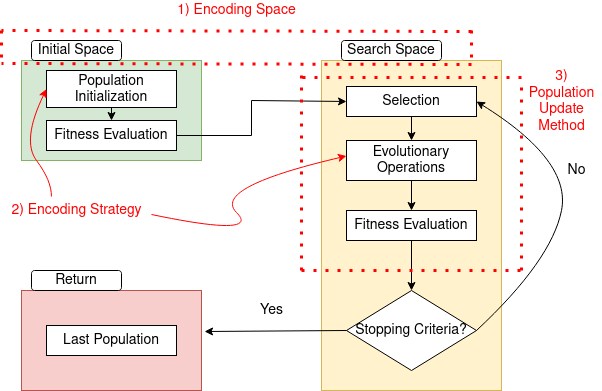
\includegraphics[scale=0.4]{evol}
    \caption{
        Generic flowchart of a typical ENAS algorithm. The white boxes show concrete steps in the algorithm's
        implementation. The enumerated red keywords are the terms used to define ENAS algorithms, and they are used
        in this figure to illustrate which steps in the algorithm belong to which terms, since they are explored
        later in this work.
    }
    \label{evol}
\end{figure}

ENAS algorithms are NAS algorithms that leverage existing evolutionary computational methods
to search for an optimal architecture within a defined search space. It can be broken
down into a series of steps exemplified by Fig. \ref{evol}.
The term \textit{population} seen in Fig. \ref{evol} is defined as a finite number of \textit{individuals},
where each individual is one neural architecture within the defined search space.

At the beginning of the algorithm an initial population is created within a pre-defined initial space.
Then, their fitnesses are evaluated, which essentially is the process of
performance estimation already covered in section \ref{PES}.

Now, this population undergoes a process that includes in sequential order:
A) \textit{selection}, B) \textit{evolutionary operations} and C) \textit{fitness evaluation}. These
steps can be broadly grouped into the \textit{population update method}, which will later be explored in
section \ref{pop}. The general concept of this phase is the core of evolutionary methods. Inspired by
the evolutionary processes in nature, a selection criteria is imposed on a given population, determining which
individuals advance to the next generation. Following that, evolutionary operations are applied to these survivors.
These mimic different concepts such as mutation, crossovers and many others to change the current architectures
and continue the search efficiently. Finally, the new changed individuals have their fitness evaluated.
If the resulting population meet the defined goal, the final architecture has been found.
Otherwise this process will be repeated using the last generation until the criteria is met.

It is possible to differentiate ENAS algorithms through four dimensions \cite{liu2021survey}:
Encoding Space, Encoding Strategy, Population Update Method and Fitness Evaluation. Fitness evaluation has however been
covered already in section \ref{PES}, therefore the focus will remain on the first three categories.

In the following subsections, state-of-the-art ENAS methods will be discussed through these different elements.
Although, ENAS encompasses many different techniques, this work will focus mostly on EA,
since the vast majority of relevant ENAS research has utilized it.

\subsubsection{Encoding Space}
The encoding space contains all the valid individuals or architectures encoded in the population \cite{liu2021survey}.
It can be further divided into the initial space and the search space, as seen in red illustrated in Fig. \ref{evol}. These two may be the same in some cases,
but often are not. The initial space is the set of all possible architectures that any individual in the initial population may
be initialized as. There are three types of architecture initialization approaches \cite{liu2021survey}:

\begin{itemize}
    \item \textbf{Starting from trivial conditions}: This method aims to impose little to no human bias in the initial
     population. The groundbreaking work in \cite{pmlr-v70-real17a} had the benefit of giving much more freedom to the algorithm
     to explore unseen architectures and also justified well the used of EC-methods instead of other approaches.
     However, this comes at the cost of high computational resources. The work in \cite{xie2017genetic} is
     also another example of competetive architecture achievements that used a trivial initial space.

    \item \textbf{Rich Initialization}: This technique, also named \textit{well-designed space}, consists of initializing
    the population within a set of state-of-the-art architectures. This way, a good architecture can be found early on
    and potentially decrease search time. On the other hand, finding novel architectures is very improbable. There has been
    relevant work that used this method as initialization technique, such as from \cite{fujino2017deep}.

    \item \textbf{Random Initialization}: This form of initialization also aims to reduce human bias or intervention in
     the process of architecture evolution. Many efforts have utilized this method such as \cite{sun2019evolving} and
     \cite{sun2019completely}. Here, the search space and the initial space are the same and initialization is random.
\end{itemize}

The search space and their constraints have been touched in section \ref{search}, where the concept of block-based and cell-based
search spaces have been introduced. Notable works like \cite{sun2019completely} use traditional blocks such as ResBlock, DenseBlock
and ConvBlock to further constraint the search space and facilitate architecture discovery. Other efforts such as
\cite{chen2019auto} and \cite{song2020efficient} used different basic blocks to adapt to their respective desired architecture
use-cases.

Most implementations of cell-based searches have the macro-architecture be based on human expertise and concentrated mostly
on optimizing their micro-architectures. This was done for example in \cite{real2019regularized}.

Nonetheless, there are more EA specific
parameters to consider when evaluating the search space of an ENAS algorithm. Evolutionary operators play a role in
constraining the algorithm's search space and will be touched on in more depth in section \ref{pop}. An example would be the
work of in \cite{irwin2019graph}, which did not specify explicitly the maximum depth of the
resulting architectures, but then used the algorithm's evolutionary operators to extend the individual's architectures
indefinitely if needed.

\subsubsection{Encoding Strategy}
The encoding strategy defines how network architectures are encoded into individuals. They can be typically split into
\textit{fixed-length} and \textit{variable-length} encoding strategies. These approaches differ in whether the length
of an individual varies during the evolutionary process, which is essentially the layer depth of resulting architectures.

In the fixed-length variant, all individuals have the same length during the search process. This facilitates
the process, since standard evolutionary operations are by design to be used with individuals of equal lengths. For example,
in the work of \cite{xie2017genetic}, this enabled a much easier implementation of its ENAS
algorithm, especially with the utilization of crossover. However, for fixed-length implementations, a maximum
length has to be established, which then also creates a dependency on human expertise and introduces bias.

On the other hand, the variable-length methods do not require human knowledge regarding layer depth, which creates
a potential to have a fully-automated implementation. Moreover, the greatest advantage to this approach is that the algorithm
can define more details of the architecture with greater freedom. This comes at the cost of a harder and more complex implementation,
since evolutionary operators may not be directly compatible with this encoding strategy, requiring a redesign. In addition to that,
the extra flexibility provided by this technique may also cause overly complex architectures with costly performance evaluations.
The work of \cite{sun2019evolving} is a prime example of a variable-length encoding strategy that needed to redesign its operators.

\subsubsection{Population Update Method}
\label{pop}
The population update method includes selection strategies and how evolutionary operators are applied. This will then
define how populations ultimately evolve. This is also illustrated in Fig. \ref{evol}.

Genetic Algorithm (GA)-based methods are the most popular approach among the EA techniques used in ENAS, since architecture representation is
very convenient in GA \cite{liu2021survey}. Selection is the first stage of updating the current population and can
be divided into several strategies, four of whom are widely used: Elitism, Discard worst or oldest, Roulette and
Tournament Selection.

Works such as \cite{elsken2017simple} take use of elitism, where essentially only the fittest of individuals are selected to
compose the next population. This can cause a loss of diversity, as there is a chance that similar architectures perform
similarly well and thus may cause generations to breed only akin individuals, since only the fittest are kept. This in turn,
can cause the population to fall within a local optima and not being able to explore efficiently.
Other approaches such as \cite{pmlr-v70-real17a} and \cite{zhang2019identify} discarded the oldest individual from the population,
which is also known as aging evolution. This ensures that the search does not focus on good models too early and therefore
performs a more broad search of the encoding space in comparison to non-aging evolution. There is also the possibility to
combine different strategies such as in \cite{zhu2019eena}, where both discarding the worst and the oldest were used.
Roulette selection, as the name implies, applies a probability to each invidividual according to its fitness. So, there is
a chance associated to each individual's survival. This means that any individual can theoretically be discarded independent
of performance or not. Finally, Tournament selection will chose from en equally likely sampling of individuals the single best one.

Finally, the most common operations in ENAS are crossover and mutation. Crossover needs two individuals to generate
an offspring, while mutation is applied solely to a single individual. Mutation wishes to reach the global optimum around
the individual which it is applied upon and generally introduces exploration \cite{liu2021survey}. Crossover on the other hand
contributes mainly to exploitation as it reunites different characteristics from ancestors into a single offspring \cite{liu2021survey}.

\subsection{NAS and tinyML}
\label{nasml}
Machine learning on small microcontrollers is a great ambition. TinyML is the field that answers to that challenge
and aims to provide intelligent features to even the cheapest off-the-shelf microcontrollers. This is not a
small effort as microcontrollers possess very limited resources, especially concerning memory and storage. In the following
subsections, relevant work that combined NAS algorithms within the tinyML universe will be shown.

\subsubsection{\textbf{MnasNET}}
The work in \cite{tan2019mnasnet} used a reinforcement learning based NAS algorithm to obtain architectures that
consider trade-offs between latency and accuracy. The search process included real latency information instead of
proxies through metrics such as FLOPs. Also, MnasNet developed what was called a
\textit{factorized hierarchical search space}, a block-based search space that differred from previous related-work that
focused on cells. This allowed different architectures per block, which effectively resulted better trade-offs between
accuracy and latency.
This work was able
to achieve state-of-the-art performance at the time on both ImageNet and COCO object detection within
mobile benchmarks \cite{tan2019mnasnet}.

\subsubsection{\textbf{MCUNet}}
MCUNet is a framework that shows promising results, composed of
two major components: the efficient neural architecture (TinyNAS) and the lightweight inference engine (TinyEngine) \cite{lin2020mcunet}.
The TinyNAS algorithm is a two-stage neural architecture search method, where firstly it optimizes the search space according to the
given resource constraints and then performs an ENAS algorithm to find the best architecture within this new search space.
Since the performance of NAS methods depend strongly on the search space \cite{radosavovic2020designing}, this technique
through extra constaints forces the search to consider a smaller set, where only architectures that fit the desired requirements
can be found. These requirements may be limited memory consumption, storage limits, latency and even energy usage.

MCUNet used weight sharing \cite{lin2020mcunet}, such that the time needed to train all possible individuals is drastically
reduced. The ENAS algorithm used in MCUNet uses elitism as its selection strategy, always choosing the top-20 individuals in
terms of accuracy within a given generation. Crossover is applied to generate 50 new candidates and then mutation with a
probablity of 10\% is used to generate the remaining 50. All generations are of size 100. Finally, after 30 iterations,
the fittest architecture is chosen.

In addition to that, TinyEngine implements a code generator-based compilation method that not only eliminates memory overhead, but also improves
the speed of inference as well \cite{lin2020mcunet}.
Finally, this work has shown to be able to
reduce memory usage by 2.7x and improve inference speed by 1.7-2.2
compared to TF-Lite Micro and CMSIS-NN, also decreased code size by up to 4.5X and 5.0x for TF-Lite Micro and CMSIS-NN
respectively \cite{lin2020mcunet}. MCUnet achieved state of the art performance, taking 12.5 GPU days to design a model
\cite{lin2020mcunet}. This is a great improvement compared to MnasNET, which took 40,000 GPU hours for the same
data set \cite{tan2019mnasnet} and is also faster than most NAS methods performed on regular machines.

\subsubsection{\textbf{MicroNets}}
The work \cite{banbury2021micronets} implemented a tailored differentiable NAS algorithm based on the work in DARTS
\cite{liu2018darts}, that discovered highly accurate models, while also satisfying SRAM, eFlash and latency constraints
within a given hardware architecture. Regularization terms are applied to the used NAS algorithm such that the resulting
models consider eFLash memory and produce activations that fit in the available SRAM \cite{banbury2021micronets}, whilst
aiming to achieve high accuracy results.

\section{Conclusion}
Throughout this work a brief overview of the current research on NAS has been displayed. NAS is not only
a complex optimization problem, but also one that requires significant computational resources in most applications. The
trade-offs of the mainstream approaches to NAS have also been demonstrated, whilst also highlighting efforts done with the
use of EC-based approaches.

In addition to that, different applications of NAS methods within the tinyML paradigm have been illustrated.
For IoT devices and microcontrollers it is not only needed to train models considering performance,
but also considering other parameters such as latency, memory usage and even energy preservation. Therefore, displaying
an interesting challenge, which brings however great promise to the field.

% references section
\bibliographystyle{IEEEtran}
\bibliography{refs}

%
\end{document}
